
%%% Local Variables:
%%% mode: latex
%%% TeX-master: t
%%% End:

\chapter{基于AS编址的互联网可扩展路由机制的软件路由器实现与测试}
\section{引言}
本章节主要通过软件路由器对基于AS编址的互联网可扩展路由机制进行实现和测试,通过观察搭建网络中,BGP路由表项的大小,判断CABA编址对路由可扩展性的作用。
\section{基于AS编址的互联网可扩展路由机制的实现方案}
基于AS编址的互联网可扩展路由机制的实现方案主要分三步:
\begin{enumerate}
\item 选择拓扑结构。该章节的实验选择现今网络Tier1层级\cite{tier1}的拓扑结构。Tier1的ASNs 见表\ref{tab:tier1asn},Tier1自治系统关系来源于CAIDA官网上20150201数据\onlinecite{caidaasdata}。
\item 生成配置文件。在充分了解Quagga软件路由器的配置之后,完成代码批量生成配置文件。每一个自治系统仅有一台路由器,需要定义该路由器的自治系统号,touter-id,邻居的IPv6地址和邻居的自治系统号,向外宣告嵌有自治系统号的IPv6前缀。以路由器174为例的配置文件如下:\\
    hostname bgpd\\
    password zebra\\
    log stdout\\
    line vty\\
    router bgp 174\\
     bgp router-id 0.0.1.74\\
     neighbor 11:0::d1 remote-as 209\\
     neighbor 11:1::11e remote-as 286\\
     neighbor 11:2::2bd remote-as 701\\
     neighbor 11:3::4d7 remote-as 1239\\
     neighbor 11:4::513 remote-as 1299\\
     neighbor 11:5::b0c remote-as 2828\\
     neighbor 11:6::b62 remote-as 2914\\
     neighbor 11:7::cb9 remote-as 3257\\
     neighbor 11:8::cf8 remote-as 3320\\
     neighbor 11:9::d1c remote-as 3356\\
     neighbor 11:a::1154 remote-as 4436\\
     neighbor 11:b::1587 remote-as 5511\\
     neighbor 11:c::1935 remote-as 6453\\
     neighbor 11:d::193d remote-as 6461\\
     neighbor 11:e::1a6a remote-as 6762\\
     neighbor 11:f::1b6a remote-as 7018\\
     neighbor 11:10::329c remote-as 12956\\
     address-family ipv6\\
     network 1000:0000:ae00::\/64\\
     neighbor 11:0::d1  activate\\
     neighbor 11:1::11e  activate\\
     neighbor 11:2::2bd  activate\\
     neighbor 11:3::4d7  activate\\
     neighbor 11:4::513  activate\\
     neighbor 11:5::b0c  activate\\
     neighbor 11:6::b62  activate\\
     neighbor 11:7::cb9  activate\\
     neighbor 11:8::cf8  activate\\
     neighbor 11:9::d1c  activate\\
     neighbor 11:a::1154  activate\\
     neighbor 11:b::1587  activate\\
     neighbor 11:c::1935  activate\\
     neighbor 11:d::193d  activate\\
     neighbor 11:e::1a6a  activate\\
     neighbor 11:f::1b6a  activate\\
     neighbor 11:10::329c  activate\\
     exit-address-family
\item  搭建实验网络环境,确保peer关系之间的路由器可以通信,非peer关系的路由器不能通信,不在同一个子网。
\end{enumerate}

\section{试验环境}
\subsection{Quagga软件路由器的核心思想和工作原理}

\begin{figure}
  \centering
  % Requires \usepackage{graphicx}
  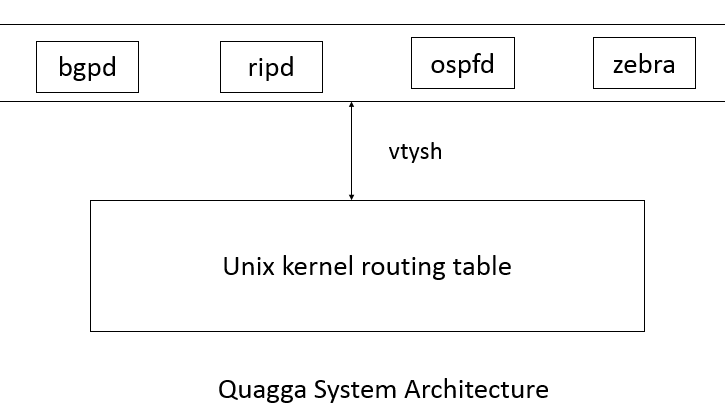
\includegraphics[width=\textwidth]{quaggastructure}\\
  \caption{QUAGGA系统结构}\label{fig:quaggastructure}
\end{figure}

Quagga\cite{quagga}软件路由器的前身是zebra,支持IPv6,不同网络协议运行不同的进程,相互独立。zebra为核心进程,管理全局路由表。网络协议进程通过vtysh进程和内核路由信息表进行交互。

\subsection{docker系统的核心思想和工作原理}
Docker\cite{docker}是通过Linux容器、直接复用本地主机的操作系统等技术实现了超轻量级的操作系统虚拟化,可以实现在一台机器上运行几千台Docker容器。在Docker中,开发人员使用镜像来构建开发容器,通过将一台配置好环境的Docker容器保存成镜像进行复用,可以快速高效的部署实验中网络环境的软件路由器。Docker中容器除了运行其中应用外,不消耗额外资源,启动时间以秒计,大量节约了开发环境的部署、实际环境的测试等时间。Docker中有三个基本概念:镜像、容器和仓库,镜像是操作系统的安装包,仓库来管理存储所有的镜像,在容器中运行镜像就实现了操作系统的功能。

\section{实验流程}
基于AS编址的互联网可扩展路由机制的软件路由器实现与测试的实验流程如下:
\begin{enumerate}
\item 确定拓扑结构:有N台路由器,每台路由器代表一个自治域。
\item 配置运行环境:安装docker软件,创建N台容器,每台容器中安装Ubuntu14.04系统,安装Quagga。
\item 配置网络环境:在本机上搭建网桥,将容器的接口与网桥的接口相连接,不同的连接配置不同局域网,每一个peer连接关系都需要在网桥上配置两个接口。
\item 生成Quagga配置文件:确定每台路由器对应的ASN,router-id,neighbor-info,network-prefix。
\item 运行Quagga中的zebra和bgpd进程,统计ipv6 bgp route的数目。
\end{enumerate}
目前实验的拓扑结构为17台路由器,17台路由器之间的peer-link连接共有149条,需要编写程序生成脚本来创建容器,启动容器,创建网桥,配置接口,启动Quagga中的进程。其中通过编写程序生成Quagga路由器BGP配置文件。
\section{实验对比设计}
单纯观察部署CABA地址方案的互联网拓扑结构生成的BGP路由表项数目,并不能说明问题。所以本章节设计了对比实验,来观察BGP路由项数目的变化趋势和变化程度。对比实验设计如下:
\begin{enumerate}
\item 给路由器配置基于AS的新型IPv6地址,向外宣布嵌入ASN的IPv6前缀。
\item 给路由器配置IPv4地址,向外宣布CAIDA官网统计出来ASN对应的所有IPv4前缀。
\end{enumerate}
\section{实验分析}
%\begin{figure}
%  \centering
%  % Requires \usepackage{graphicx}
%  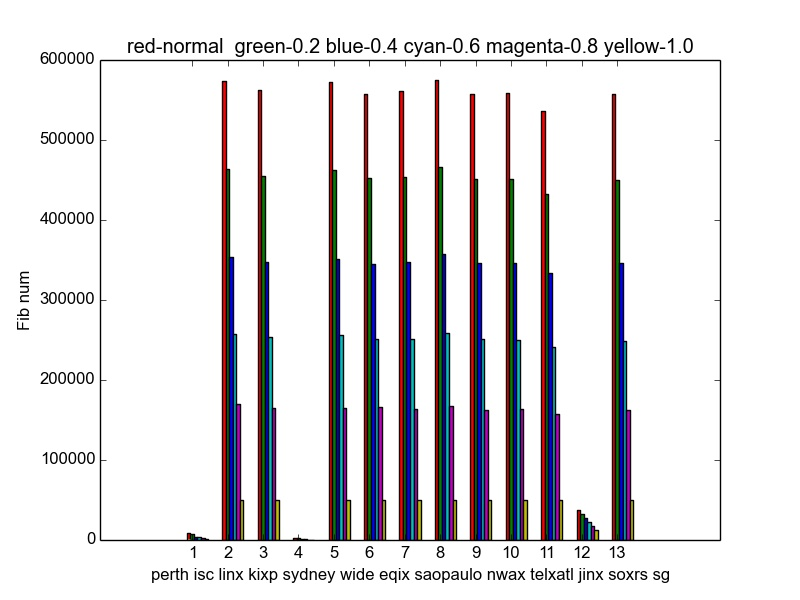
\includegraphics[width=\textwidth]{2}\\
%  \caption{软件路由器:基于CABA编址的BGP路由表表项数据}\label{fig:temp}
%\end{figure}

目前该实验基于Tier1层级的自治系统之间构成的拓扑结构,完成了给路由器配置基于AS的新型IPv6地址,向外宣布嵌入ASN的IPv6前缀的部分。:

\section{小结}
我们大胆合理推测,基于CABA编址BGP路由表项的数目将会远小于现有对应的BGP路由表项,因为基于CABA编址的BGP路由表项只需要向外宣布一条前缀,而现有网络对于一个自治系统,可能向外宣布多条前缀,最多可达4000多条,参考图\ref{fig:7}。